The goal of this chapter is to evaluate the proposed \textit{Invox} system and analyze its performance across multiple extraction strategies using the \textbf{MUC-4 benchmark dataset}. The evaluation aims to measure how effectively the system transforms unstructured, noisy text into structured templates under real-world conditions. To this end, the assessment focuses on the dimensions of \textbf{accuracy}, \textbf{consistency}, \textbf{latency}, \textbf{cost}, and \textbf{modularity}, in direct correspondence with the requirements defined in Chapter~\ref{chap:analysis}.

Unlike traditional information extraction evaluations that rely on strict lexical overlap, the MUC-4 dataset poses a distinctive challenge: both the gold standard and system predictions may include \textit{multiple valid fillers} per slot, expressed through paraphrases or partial phrases. A purely string-based comparison would therefore underestimate performance. To account for this, all evaluations employ an \textbf{embedding-based semantic framework} in which cosine similarity between gold and predicted values captures conceptual correctness rather than surface form matching. This provides a fairer, more robust measure of information extraction quality.

The chapter proceeds as follows. Section~\ref{sec:eval-dataset} introduces the MUC-4 dataset and the preprocessing pipeline applied prior to evaluation. Section~\ref{sec:eval-metrics} defines the semantic similarity metrics and auxiliary measures such as latency and cost. Section~\ref{sec:eval-setup} describes the experimental setup and the evaluated strategies. Sections~\ref{sec:eval-results}--\ref{sec:eval-comparative} present quantitative and qualitative results, followed by a summary that relates the findings to the original design requirements.

\section{Dataset and Preprocessing}
\label{sec:eval-dataset}

The \textbf{MUC-4 dataset} was introduced as part of the Message Understanding Conference (MUC) evaluation series and remains one of the most established benchmarks for information extraction in the terrorism domain. It consists of English-language newswire articles in which domain experts annotated terrorist incidents that occurred primarily in Latin America during the late 1980s. Each article may describe one or more events, and each event is represented by a structured template containing up to \textbf{24 annotated fields} that capture various attributes of the incident, including participants, timing, and contextual information.

For the purpose of this evaluation, the full schema was reduced to the subset of fields that are both semantically informative and consistently populated. The final evaluation schema includes: \texttt{incidentType}, \texttt{incidentDate}, \texttt{incidentLocation}, \texttt{incidentStage}, \texttt{perpetratorIndividual}, \texttt{perpetratorOrganization}, \texttt{target}, \texttt{victim}, and \texttt{weapon}. These correspond directly to the slots defined in the \textit{Invox} template-filling system and reflect the most important aspects of event understanding. This reduction enables a focused evaluation of the system’s ability to extract the key components of each incident rather than peripheral metadata.

Each article in MUC-4 can contain multiple annotated events. To align with the design of the \textit{Invox} pipeline—where each input corresponds to a single structured template—the evaluation considers only one event per document. When multiple event templates are available, the preprocessing procedure automatically selects the most complete annotation, typically the first one with non-empty values across the selected fields. This ensures a one-to-one correspondence between document text and evaluated template, which simplifies both comparison and interpretation.

\subsection{Preprocessing}

The preprocessing pipeline is applied exclusively to the \textbf{gold annotations} provided by the MUC-4 dataset, as the system outputs generated by \textit{Invox} already conform to the standardized schema. The original MUC-4 corpus is distributed in two complementary formats: 
(1) \textit{value files}, which contain the full article texts along with document identifiers, and 
(2) \textit{key files}, which contain the corresponding event templates with up to 24 annotated fields for each document. 
To construct a consistent evaluation dataset, these two sources were combined into a unified JSON representation in which each document entry contains both the raw text and the corresponding gold template.

Once the text–template pairs were combined, a sequence of normalization and filtering steps was applied to clean and harmonize the annotations:

\begin{itemize}
    \item \textbf{Schema normalization:} all gold templates were converted into a unified JSON structure using the standardized field names: \texttt{incidentType}, \texttt{incidentDate}, \texttt{incidentLocation}, \texttt{incidentStage}, \texttt{perpetratorIndividual}, \texttt{perpetratorOrganization}, \texttt{target}, \texttt{victim}, and \texttt{weapon}. Fields outside this subset were discarded.
    \item \textbf{Event filtering:} each MUC-4 document can include multiple annotated events. To ensure compatibility with the \textit{Invox} workflow, where each input corresponds to a single structured template, only one event per document was retained. The selection heuristic prioritized the event with the most complete slot coverage (i.e., the greatest number of non-empty fields).
    \item \textbf{Text normalization:} all article texts were lowercased, punctuation standardized, and redundant whitespace removed to facilitate reliable tokenization and embedding consistency during evaluation.
    \item \textbf{Placeholder cleaning:} annotation placeholders such as ``--'', ``N/A'', or empty markers were removed from the gold templates to prevent artificial mismatches during similarity computation.
    \item \textbf{Deduplication of fillers:} repeated mentions of the same entity within a field (for example, a perpetrator organization listed multiple times) were collapsed into unique entries to avoid double counting.
\end{itemize}

After these operations, each document was represented as a normalized JSON object containing one cleaned article text and a single corresponding event template. The processed dataset includes approximately \textbf{1,300 examples} derived from the original MUC-4 training and development files, which were used to populate the retrieval index and provide exemplars for the RAG module. A separate subset of \textbf{100 held-out examples} was reserved for evaluation and served as the test set for measuring extraction quality. 

This preprocessing ensures a harmonized dataset structure that faithfully preserves the original semantic content while enabling consistent embedding-based comparison between gold annotations and the structured templates generated by the \textit{Invox} system.


\subsection{Schema Caveats for Slot Filling}

While MUC-4 is a classic benchmark, its slot schema introduces mismatches that matter in practice. A single article often mentions several incidents, yet the template expects one event, forcing systems to choose which facts to keep and which to drop. Roles can be underspecified or mixed—generic actors like “rebels” appear alongside named groups and people—so the split between \texttt{perpetratorIndividual} and \texttt{perpetratorOrganization} is frequently ambiguous. Granularity also varies by field: locations oscillate between country–city–neighborhood and just a country; weapons range from specific (“car bomb”) to coarse (“explosive”) or even dashes; dates are sometimes relative in text (“yesterday”) but absolute in gold. These inconsistencies create false errors for otherwise sensible fills.

A second issue is calibration and evidence. Gold templates sometimes omit entities that are clearly in the text, and at other times include fillers that are only implied (e.g., an organization named via allegation). This rewards systems that guess and penalizes ones that abstain without confirmation. Combined with translation/OCR artifacts (casing, accents, bracketed notes), exact-match scoring can overstate mistakes. Our setup mitigates this with normalization, soft/semantic matching, and an explicit fill-vs-abstain decision, but these schema quirks remain important when interpreting scores and designing post-processing.

\section{Evaluation Metrics}
\label{sec:eval-metrics}

We evaluate \textit{Invox} along complementary axes: (i) semantic accuracy under paraphrase and set-size mismatch, (ii) behavior under typed schema constraints, and (iii) operational efficiency. 
Because MUC-4 slots often admit paraphrases or near-synonyms, we use embedding-based measurements for text and list fields, while keeping exact comparison for typed slots (enums, dates).
To disentangle empty-field effects, we report results in two regimes:
\emph{baseline} (standard scoring, where gold-empty $\wedge$ pred-empty contributes positively) and 
\emph{gold-nonempty-only} (scores computed \emph{only} when the gold slot is nonempty).

\subsection{Embedding-Based Accuracy (R2)}
\label{subsec:emb-acc}

For text and list-valued slots, we compare unordered sets of fillers using sentence embeddings (\texttt{all-MiniLM-L6-v2}) and cosine similarity. 
Let $G=\{g_i\}$ and $P=\{p_j\}$ be the gold and predicted sets. 
We define gold-anchored recall and prediction-anchored precision surrogates:
\begin{align}
\text{SoftCoverage}   &= \frac{1}{|G|}\sum_{i}\max_{j}\ \cos\!\big(\mathrm{enc}(g_i),\,\mathrm{enc}(p_j)\big), \\
\text{SoftSpecificity} &= \frac{1}{|P|}\sum_{j}\max_{i}\ \cos\!\big(\mathrm{enc}(p_j),\,\mathrm{enc}(g_i)\big).
\end{align}

Their symmetric mean gives a threshold-free Chamfer similarity,
\[
\text{Chamfer} \;=\; \tfrac{1}{2}\big(\text{SoftCoverage}+\text{SoftSpecificity}\big),
\]
and we also report a \emph{Soft-F1} (\textbf{SF1}) as the harmonic mean of SoftCoverage and SoftSpecificity:
\[
\text{SF1} \;=\; \frac{2\,\text{SoftCoverage}\cdot\text{SoftSpecificity}}{\text{SoftCoverage}+\text{SoftSpecificity}}.
\]
For \textbf{enums} and \textbf{dates}, we use \emph{exact} scoring (match = 1, otherwise 0), aligning with the typed nature of these slots. 
Free-form \textbf{locations} are treated as text (singletons) and scored via embeddings.

\paragraph{Two scoring regimes.} 
We compute all scores twice: (i) \textbf{baseline} (standard), and (ii) \textbf{gold-nonempty-only} (ignores any (doc,slot) where the gold is empty). 
This separation isolates true content quality from empty-field advantages.

\subsection{Decision Quality Under Typed Constraints (R1)}
\label{subsec:consistency}

Beyond similarity, we evaluate the model's \emph{fill decision} with a presence matrix over four outcomes per slot: 
gold-empty/pred-empty, gold-empty/pred-nonempty, gold-nonempty/pred-empty, gold-nonempty/pred-nonempty. 
From this we derive compact decision metrics:
\begin{itemize}
  \item \textbf{FDA} (Fill-Decision Accuracy): fraction of cases where the empty vs.\ nonempty choice matches gold.
  \item \textbf{HR} (Hallucination Rate): $\Pr(\text{pred nonempty} \mid \text{gold empty})$.
  \item \textbf{MR} (Missing Rate): $\Pr(\text{pred empty} \mid \text{gold nonempty})$.
  \item \textbf{RFA} (Required-Fill Accuracy): average slot score \emph{conditioned} on gold-nonempty \emph{and} pred-nonempty, capturing content quality when the model commits to a fill.
\end{itemize}
To summarize empty-field sensitivity we report the \textbf{Empty Advantage Index (EAI)}:
\[
\text{EAI} \;=\; \text{OBS} - \text{NES},
\]
where \textbf{OBS} is the overall baseline score and \textbf{NES} is the overall score in the gold-nonempty-only regime (\S\ref{sec:results}). 
Higher EAI indicates stronger reliance on empty$\leftrightarrow$empty matches.



\subsection{Latency and Cost at Inference (R6)}
\label{subsec:latency-cost}

Operational efficiency is measured per document from \texttt{timing.duration\_ms}, reporting p50 (median), p90, p95, p99, mean, min, and max. 
When available, we also estimate cost from API token usage (prompts, completions, and embeddings), reported as USD per document. 
Because retrieval and embedding are lightweight relative to decoding, schema- and example-guided approaches remain compatible with near real-time use.

\subsection{User Correction and Human-in-the-Loop Reliability (R4)}
\label{subsec:correction}

Although MUC-4 does not capture interactive editing, \textit{Invox} surfaces all auto-filled fields for review with typed widgets (date pickers, enum selectors, multi-value inputs). 
This design safely combines ``empty-when-uncertain'' behavior with rapid human confirmation, preserving downstream data quality.

\subsection{Modularity and Extensibility (R5)}
\label{subsec:modularity}

The architecture decouples retrieval, prompting, decoding, and verification into swappable modules. 
We evaluate alternative extraction strategies under the same metrics (OBS/NES/EAI, SF1/Chamfer, FDA/HR/MR/RFA, latency), enabling targeted optimization. 
Because slots are declarative (descriptions, types, allowed values), new domains or fields integrate without changing the evaluation stack.

\paragraph{Summary.}
Our protocol reports (i) \textbf{content similarity} (SoftCoverage, SoftSpecificity, Chamfer, SF1), (ii) \textbf{decision quality} (FDA, HR, MR, RFA) with an empty-field sensitivity index (EAI), under both \textbf{baseline} and \textbf{gold-nonempty-only} regimes, and (iii) \textbf{operational efficiency} (latency, cost). 
Together these satisfy requirements on accuracy (R2), consistency (R1), domain alignment (R3), modularity (R5), operational efficiency (R6), and human oversight (R4) in a single, coherent evaluation framework.

\section{Experimental Setup}
\label{sec:eval-setup}

This section describes the configuration of the experiments conducted to evaluate the \textit{Invox} system under different orchestration strategies. All evaluations were executed using the preprocessed MUC-4 dataset described in Section~\ref{sec:eval-dataset} and the embedding-based metrics defined in Section~\ref{sec:eval-metrics}.  
The setup ensures comparability across strategies by maintaining identical model parameters, embedding configurations, and evaluation scripts.

\subsection{Compared Strategies}

The \textit{Invox} system supports multiple extraction strategies that differ in how they allocate reasoning effort across large-language-model (LLM) calls. Each strategy is evaluated independently but within the same pipeline, demonstrating the modular nature of the architecture.  

\begin{itemize}
    \item \textbf{S1: Single-Pass Full Input} — the entire document is processed in a single inference step using one LLM instance. This approach minimizes latency and cost but provides limited internal verification.
    \item \textbf{S2: Iterative Single-Field} — each field is extracted sequentially in separate LLM calls. This allows focused reasoning for difficult slots such as \texttt{perpetratorIndividual} or \texttt{target}, often improving precision at the cost of longer inference time.
    \item \textbf{S3: Multi-LLM Consensus (Full)} — multiple LLMs (e.g., GPT-5 and Gemini 2.5) process the entire input independently. The Verification Agent aggregates their results via consensus scoring to improve overall reliability.
    \item \textbf{S4: Multi-LLM Per-Field} — similar to S3 but the consensus process operates at the field level, combining specialized model outputs per slot. This configuration provides the most granular control over extraction quality.
    \item \textbf{S5: LangExtract Baseline} — a non-LLM rule-based extraction pipeline used as an external baseline. It relies on handcrafted patterns and regular expressions and serves to contextualize the semantic improvements achieved by \textit{Invox}.
\end{itemize}

All strategies share the same input format and produce outputs following the schema 
(\texttt{incidentType}, \texttt{incidentDate}, \texttt{incidentLocation}, \texttt{incidentStage}, \texttt{perpetratorIndividual}, \texttt{perpetratorOrganization}, \texttt{target}, \texttt{victim}, \texttt{weapon}).  
This unified design enables a direct, component-wise comparison of accuracy, latency, and cost.

\subsection{Embedding Models}

Semantic similarity between predicted and reference fillers is computed using the \texttt{sentence-transformers} library.  
The primary encoder is \texttt{all-MiniLM-L6-v2}, chosen for its balance between speed and representational quality.  
To verify metric robustness, a secondary encoder, \texttt{multi-qa-MiniLM-L6-cos-v1}, was used for cross-checking.  
Both models produce 384-dimensional embeddings normalized to unit length, ensuring that cosine similarity values fall within the range [0, 1].  
Empirical tests showed that the two encoders produce nearly identical ranking orders across strategies, confirming the stability of the evaluation results.

\subsection{Environment and Settings}

All experiments were run on a CPU-only Ubuntu 24.04.3 LTS machine (kernel 6.14) with an Intel i7-6600U (2 cores, 4 threads), 16\,GB RAM, and integrated Intel HD 520 graphics (no discrete NVIDIA GPU / no CUDA). Local preprocessing and evaluation were implemented in Python~3.10; the orchestration service was built with Node.js~20 (TypeScript).

Model inference used hosted APIs (OpenAI, Gemini) with deterministic settings (\texttt{temperature=0.2}, \texttt{top-p=1.0}) and fixed random seeds for reproducibility. Latency was measured at the API boundary per document (request--response wall time, including network). Token usage and provider-reported pricing were logged to estimate cost. All strategies used identical batching and concurrency to avoid scheduling bias.

\section{Results – LangExtract Baseline (S5)}
\label{sec:eval-langextract}

\textbf{LangExtract} is an open-source, LLM-powered Python library for schema-constrained extraction. 
In our pipeline it serves as a deterministic orchestration wrapper around model calls (strict JSON schema, span grounding).

\subsection*{Quantitative Results}

\begin{table}[H]
    \centering
    \caption{Headline metrics for LangExtract on MUC-4 ($N{=}100$ documents).}
    \label{tab:langextract-headline}
    \begin{tabular}{lcccccccc}
        \toprule
        OBS & NES & EAI & SF1\,(base) & SF1\,(nonempty) & FDA & HR & MR & RFA \\
        \midrule
        0.684 & 0.502 & 0.182 & 0.653 & 0.406 & 0.756 & 0.088 & 0.369 & 0.796 \\
        \bottomrule
    \end{tabular}
\end{table}

\begin{table}[H]
    \centering
    \caption{Per-field average scores for LangExtract (baseline regime; $N{=}100$).}
    \label{tab:langextract-perfield}
    \begin{tabular}{lcc}
        \toprule
        Field & Average Score & \#Docs \\
        \midrule
        incidentType & 0.880 & 100 \\
        incidentDate & 0.570 & 100 \\
        incidentLocation & 0.512 & 100 \\
        incidentStage & 0.830 & 100 \\
        perpetratorIndividual & 0.719 & 100 \\
        perpetratorOrganization & 0.681 & 100 \\
        target & 0.523 & 100 \\
        victim & 0.596 & 100 \\
        weapon & 0.844 & 100 \\
        \midrule
        \textbf{Overall Average (OBS)} & \textbf{0.684} & \textbf{900 comps} \\
        \bottomrule
    \end{tabular}
\end{table}

\begin{table}[H]
    \centering
    \caption{Embedding metrics (overall) for LangExtract.}
    \label{tab:langextract-embed-overall}
    \begin{tabular}{lccc}
        \toprule
        Regime & Soft-Coverage & Soft-Specificity & Chamfer (Sym.) \\
        \midrule
        Baseline & 0.646 & 0.661 & 0.653 \\
        Gold-nonempty-only & 0.391 & 0.421 & 0.406 \\
        \bottomrule
    \end{tabular}
\end{table}

\begin{table}[H]
    \centering
    \caption{Per-field embedding metrics for LangExtract (baseline; text/list fields).}
    \label{tab:langextract-embed-perfield}
    \begin{tabular}{lccc}
        \toprule
        Field & Soft-Coverage & Soft-Specificity & Chamfer \\
        \midrule
        incidentLocation & 0.512 & 0.512 & 0.512 \\
        perpetratorIndividual & 0.719 & 0.730 & 0.724 \\
        perpetratorOrganization & 0.681 & 0.679 & 0.680 \\
        target & 0.523 & 0.531 & 0.527 \\
        victim & 0.596 & 0.660 & 0.628 \\
        weapon & 0.844 & 0.854 & 0.849 \\
        \bottomrule
    \end{tabular}
\end{table}

\subsection*{Latency Analysis}

\begin{table}[H]
    \centering
    \caption{Latency statistics for LangExtract (seconds).}
    \label{tab:langextract-latency}
    \begin{tabular}{lccccccc}
        \toprule
        p50 & p90 & p95 & p99 & Mean & Min & Max \\
        \midrule
        21.15 & 57.61 & 65.39 & 99.19 & 27.03 & 1.95 & 109.84 \\
        \bottomrule
    \end{tabular}
\end{table}

\subsection*{Insights}

\begin{itemize}
    \item \textbf{Strong, conservative filler.} Very low HR (0.088) and high RFA (0.796): when it fills, it’s usually good; it avoids over-filling.
    \item \textbf{Nonempty quality lags.} The gap (EAI $=0.182$) shows reliance on empty$\leftrightarrow$empty matches; NES (0.502) and SF1\,(nonempty) (0.406) are notably lower.
    \item \textbf{Field skew.} Best on \texttt{incidentType}/\texttt{weapon}/\texttt{stage}; weaker on \texttt{target}, \texttt{location}, and especially \texttt{perpetratorOrganization} under gold-nonempty evaluation.
    \item \textbf{Dates under-filled.} Gold-nonempty \texttt{incidentDate} averaged 0.000 and the confusion table shows abstention when gold is nonempty (43 misses), explaining part of the MR (0.369).
    \item \textbf{Runtime is moderate.} Median $\sim$21\,s with a long tail; practical for batch or async passes.
\end{itemize}

\section{Results – Strategy S1: Single-Pass Full Input}
\label{sec:eval-s1}

The \textbf{S1: Single-Pass Full Input} configuration extracts all nine MUC-4 slots in a single LLM call. 
We evaluate three S1 variants: 
\textbf{S1.0} = no few-shot examples on the original MUC-4 dataset; 
\textbf{S1.1} = with few-shot examples on the original dataset; 
\textbf{S1.2} = with few-shot examples on a modified MUC-4 dataset that mimics speech-style transcripts.

\subsection*{Headline Results}


\begin{figure}[h]
\centering
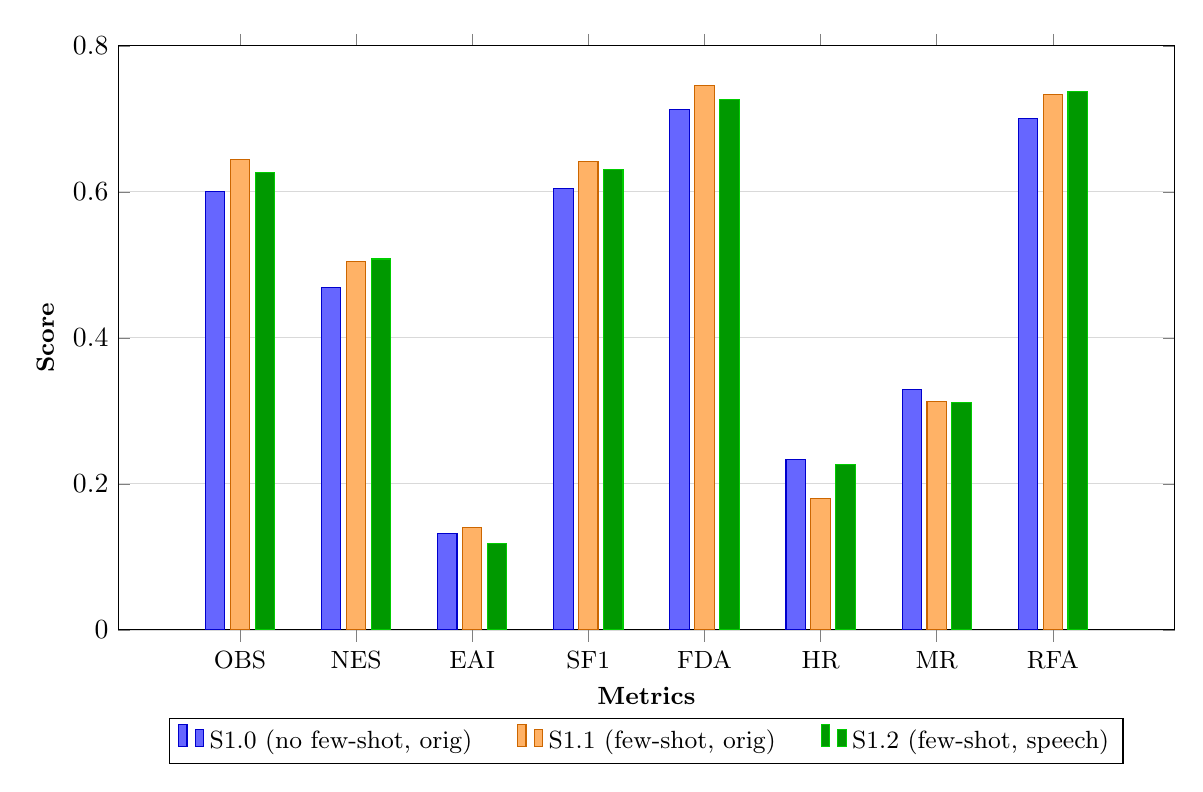
\begin{tikzpicture}
  \begin{axis}[
    width=15cm,
    height=9cm,
    ybar,
    bar width=7pt,
    ylabel={Score},
    ylabel style={font=\small\bfseries},
    xlabel={Metrics},
    xlabel style={font=\small\bfseries},
    symbolic x coords={OBS, NES, EAI, SF1, FDA, HR, MR, RFA},
    xtick=data,
    xticklabel style={font=\small},
    ymin=0,
    ymax=0.8,
    ytick={0, 0.2, 0.4, 0.6, 0.8},
    ymajorgrids=true,
    grid style={line width=0.3pt, draw=gray!30},
    legend style={
      at={(0.5,-0.15)},
      anchor=north,
      legend columns=3,
      font=\small,
      /tikz/every even column/.append style={column sep=0.5cm}
    },
    enlarge x limits=0.15,
  ]
  
  % S1.0 (no few-shot, orig) - Blue
  \addplot[fill=blue!60, draw=blue!80!black] coordinates {
    (OBS, 0.601)
    (NES, 0.469)
    (EAI, 0.132)
    (SF1, 0.604)
    (FDA, 0.713)
    (HR, 0.233)
    (MR, 0.329)
    (RFA, 0.700)
  };
  \addlegendentry{S1.0 (no few-shot, orig)}
  
  % S1.1 (few-shot, orig) - Orange
  \addplot[fill=orange!60, draw=orange!80!black] coordinates {
    (OBS, 0.644)
    (NES, 0.504)
    (EAI, 0.140)
    (SF1, 0.642)
    (FDA, 0.746)
    (HR, 0.180)
    (MR, 0.313)
    (RFA, 0.733)
  };
  \addlegendentry{S1.1 (few-shot, orig)}
  
  % S1.2 (few-shot, speech) - Green
  \addplot[fill=green!60!black, draw=green!80!black] coordinates {
    (OBS, 0.626)
    (NES, 0.508)
    (EAI, 0.118)
    (SF1, 0.631)
    (FDA, 0.727)
    (HR, 0.226)
    (MR, 0.311)
    (RFA, 0.738)
  };
  \addlegendentry{S1.2 (few-shot, speech)}
  
  \end{axis}
\end{tikzpicture}
\caption{Headline metrics for S1 variants on MUC-4 ($N{=}100$).}
\label{fig:s1-variants-bar}
\end{figure}

\paragraph{Per-field (reference for S1.1).}
\texttt{perpetratorOrganization} and \texttt{weapon} lead; \texttt{perpetratorIndividual} and \texttt{incidentLocation} remain harder.

\begin{table}[H]
    \centering
    \caption{Per-field average scores for S1.1 ($N{=}100$).}
    \label{tab:s1-perfield}
    \begin{tabular}{lcc}
        \toprule
        Field & Avg.\ Score & \#Docs \\
        \midrule
        incidentType & 0.510 & 100 \\
        incidentDate & 0.760 & 100 \\
        incidentLocation & 0.516 & 100 \\
        incidentStage & 0.710 & 100 \\
        perpetratorIndividual & 0.584 & 100 \\
        perpetratorOrganization & 0.752 & 100 \\
        target & 0.592 & 100 \\
        victim & 0.563 & 100 \\
        weapon & 0.807 & 100 \\
        \midrule
        \textbf{Overall (OBS)} & \textbf{0.644} & \textbf{900 comps} \\
        \bottomrule
    \end{tabular}
\end{table}

\subsection*{Latency}

\begin{figure}[H]
\centering
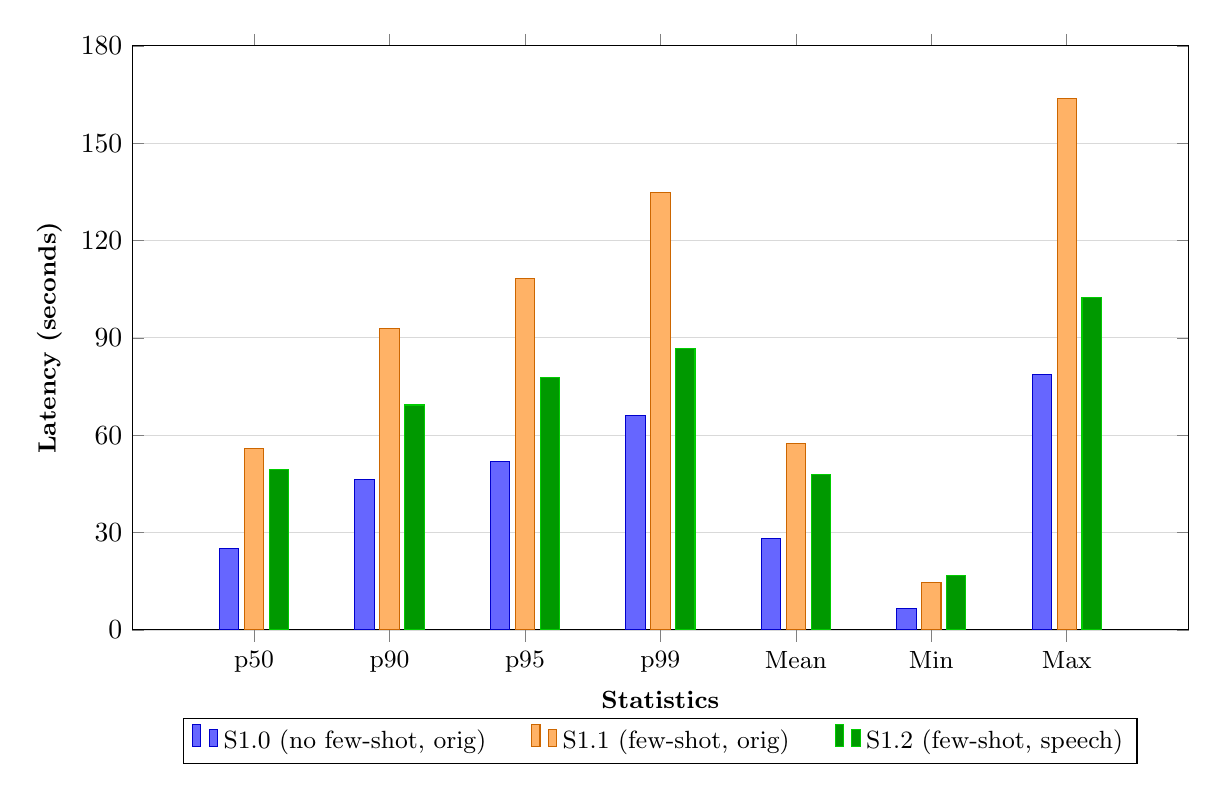
\begin{tikzpicture}
  \begin{axis}[
    width=15cm,
    height=9cm,
    ybar,
    bar width=7pt,
    ylabel={Latency (seconds)},
    ylabel style={font=\small\bfseries},
    xlabel={Statistics},
    xlabel style={font=\small\bfseries},
    symbolic x coords={p50, p90, p95, p99, Mean, Min, Max},
    xtick=data,
    xticklabel style={font=\small},
    ymin=0,
    ymax=180,
    ytick={0, 30, 60, 90, 120, 150, 180},
    ymajorgrids=true,
    grid style={line width=0.3pt, draw=gray!30},
    legend style={
      at={(0.5,-0.15)},
      anchor=north,
      legend columns=3,
      font=\small,
      /tikz/every even column/.append style={column sep=0.5cm}
    },
    enlarge x limits=0.15,
  ]
  
  % S1.0 (no few-shot, orig) - Blue
  \addplot[fill=blue!60, draw=blue!80!black] coordinates {
    (p50, 25.04)
    (p90, 46.49)
    (p95, 51.82)
    (p99, 66.12)
    (Mean, 28.17)
    (Min, 6.51)
    (Max, 78.65)
  };
  \addlegendentry{S1.0 (no few-shot, orig)}
  
  % S1.1 (few-shot, orig) - Orange
  \addplot[fill=orange!60, draw=orange!80!black] coordinates {
    (p50, 55.91)
    (p90, 93.01)
    (p95, 108.40)
    (p99, 134.93)
    (Mean, 57.34)
    (Min, 14.54)
    (Max, 163.79)
  };
  \addlegendentry{S1.1 (few-shot, orig)}
  
  % S1.2 (few-shot, speech) - Green
  \addplot[fill=green!60!black, draw=green!80!black] coordinates {
    (p50, 49.36)
    (p90, 69.30)
    (p95, 77.84)
    (p99, 86.79)
    (Mean, 47.89)
    (Min, 16.85)
    (Max, 102.50)
  };
  \addlegendentry{S1.2 (few-shot, speech)}
  
  \end{axis}
\end{tikzpicture}
\caption{Latency statistics for S1 variants (seconds).}
\label{fig:s1-latency-bar}
\end{figure}

\subsection*{Insights}

\begin{itemize}
    \item \textbf{Few-shot boosts the single-pass baseline.} Moving from S1.0 to S1.1 improves OBS (+0.043) and SF1 (+0.038), increases FDA (0.713$\rightarrow$0.746), and cuts HR (0.233$\rightarrow$0.180). Gains concentrate in entity-rich fields (\texttt{perpetratorOrganization}, \texttt{weapon}) and reduce empty-field errors.
    \item \textbf{Speech-style inputs remain robust.} S1.2 trails S1.1 modestly on OBS/SF1 but achieves the best NES (0.508) and RFA (0.738), indicating strong content quality when gold is nonempty and both sides fill. Its lower EAI (0.118) suggests less dependence on empty-field advantage.
    \item \textbf{Decision behavior stabilizes with few-shot.} Few-shot lowers hallucination rate (HR) and raises fill-decision accuracy (FDA). S1.2 keeps FDA competitive (0.727) with the lowest missing rate (MR{=}0.311, tie within rounding), despite noisier inputs.
    \item \textbf{Consistent hard spots.} \texttt{perpetratorIndividual} remains the most difficult (sparse gold, high MR in nonempty regime); \texttt{incidentLocation} shows moderate improvements but stays challenging compared to \texttt{weapon}/\texttt{perpetratorOrganization}.
    \item \textbf{Latency–quality trade-off and overall choice.} S1.0 is fastest (p50 $\sim$25\,s/doc) but least accurate. S1.1 is the strongest accuracy baseline on clean text (p50 $\sim$56\,s/doc) at higher latency. S1.2 offers a middle ground for speech-like inputs—near S1.1 quality with shorter tails (p99 86.8\,s vs.\ 134.9\,s)—and is a sensible default when spoken-text robustness matters.
\end{itemize}

\section{Results – Strategy S2: Iterative Single-Field}
\label{sec:eval-s2}

The \textbf{S2: Iterative Single-Field} strategy fills the template sequentially, invoking the LLM once per slot.
We evaluate three S2 variants:
\textbf{S2.0} = no few-shot examples on the original MUC-4 dataset;
\textbf{S2.1} = with few-shot examples on the original dataset;
\textbf{S2.2} = with few-shot examples on a modified dataset that mimics speech-style transcripts.

\subsection*{Headline Results}

\begin{figure}[h]
\centering
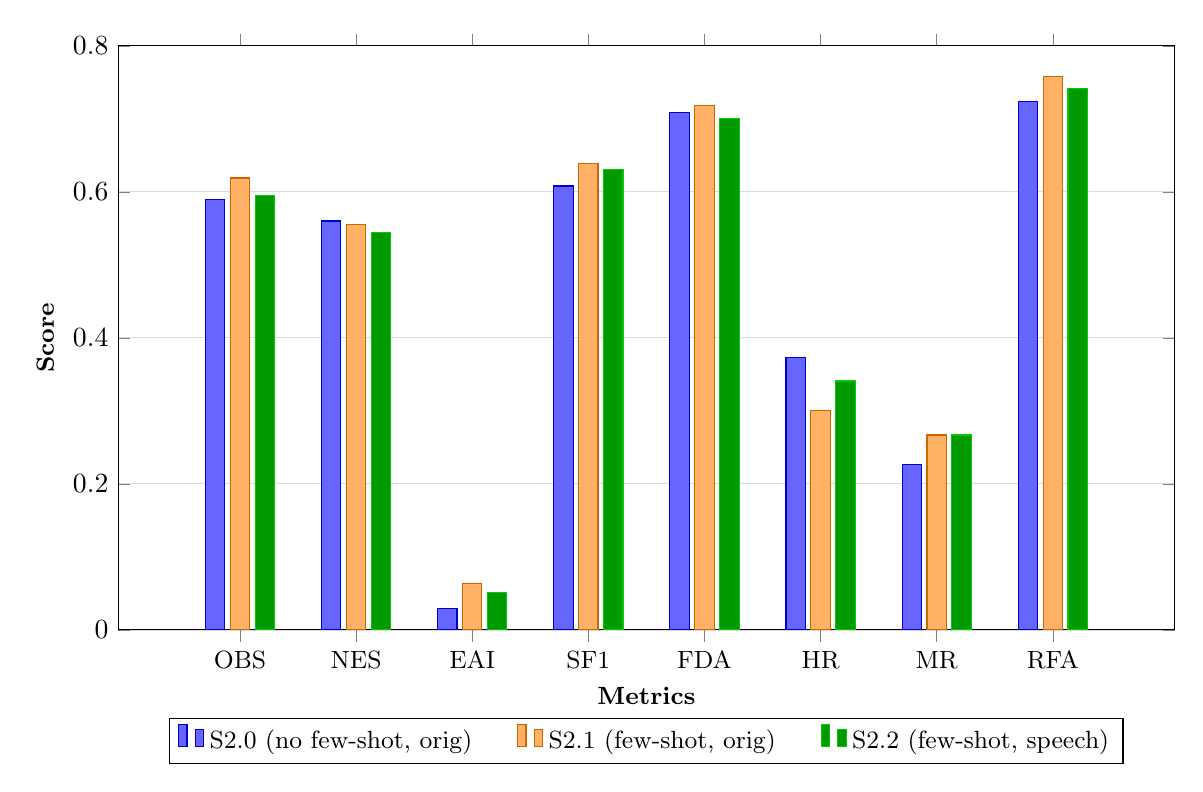
\begin{tikzpicture}
  \begin{axis}[
    width=15cm,
    height=9cm,
    ybar,
    bar width=7pt,
    ylabel={Score},
    ylabel style={font=\small\bfseries},
    xlabel={Metrics},
    xlabel style={font=\small\bfseries},
    symbolic x coords={OBS, NES, EAI, SF1, FDA, HR, MR, RFA},
    xtick=data,
    xticklabel style={font=\small},
    ymin=0,
    ymax=0.8,
    ytick={0, 0.2, 0.4, 0.6, 0.8},
    ymajorgrids=true,
    grid style={line width=0.3pt, draw=gray!30},
    legend style={
      at={(0.5,-0.15)},
      anchor=north,
      legend columns=3,
      font=\small,
      /tikz/every even column/.append style={column sep=0.5cm}
    },
    enlarge x limits=0.15,
  ]
  
  % S2.0 (no few-shot, orig) - Blue
  \addplot[fill=blue!60, draw=blue!80!black] coordinates {
    (OBS, 0.590)
    (NES, 0.560)
    (EAI, 0.029)
    (SF1, 0.608)
    (FDA, 0.709)
    (HR, 0.373)
    (MR, 0.226)
    (RFA, 0.724)
  };
  \addlegendentry{S2.0 (no few-shot, orig)}
  
  % S2.1 (few-shot, orig) - Orange
  \addplot[fill=orange!60, draw=orange!80!black] coordinates {
    (OBS, 0.619)
    (NES, 0.555)
    (EAI, 0.064)
    (SF1, 0.639)
    (FDA, 0.718)
    (HR, 0.301)
    (MR, 0.267)
    (RFA, 0.758)
  };
  \addlegendentry{S2.1 (few-shot, orig)}
  
  % S2.2 (few-shot, speech) - Green
  \addplot[fill=green!60!black, draw=green!80!black] coordinates {
    (OBS, 0.595)
    (NES, 0.544)
    (EAI, 0.051)
    (SF1, 0.631)
    (FDA, 0.700)
    (HR, 0.341)
    (MR, 0.267)
    (RFA, 0.742)
  };
  \addlegendentry{S2.2 (few-shot, speech)}
  
  \end{axis}
\end{tikzpicture}
\caption{Headline metrics for S2 variants on MUC-4 ($N{=}100$).}
\label{fig:s2-variants-bar}
\end{figure}

\paragraph{Per-field (reference for S2.1).}
\texttt{perpetratorOrganization} and \texttt{weapon} are strongest; \texttt{perpetratorIndividual} remains difficult; \texttt{incidentLocation} benefits from per-slot prompting.

\begin{table}[H]
    \centering
    \caption{Per-field average scores for S2.1 ($N{=}100$).}
    \label{tab:s2-perfield}
    \begin{tabular}{lcc}
        \toprule
        Field & Avg.\ Score & \#Docs \\
        \midrule
        incidentType & 0.520 & 100 \\
        incidentDate & 0.550 & 100 \\
        incidentLocation & 0.597 & 100 \\
        incidentStage & 0.700 & 100 \\
        perpetratorIndividual & 0.564 & 100 \\
        perpetratorOrganization & 0.738 & 100 \\
        target & 0.608 & 100 \\
        victim & 0.543 & 100 \\
        weapon & 0.751 & 100 \\
        \midrule
        \textbf{Overall (OBS)} & \textbf{0.619} & \textbf{900 comps} \\
        \bottomrule
    \end{tabular}
\end{table}

\subsection*{Latency}

\begin{figure}[H]
\centering
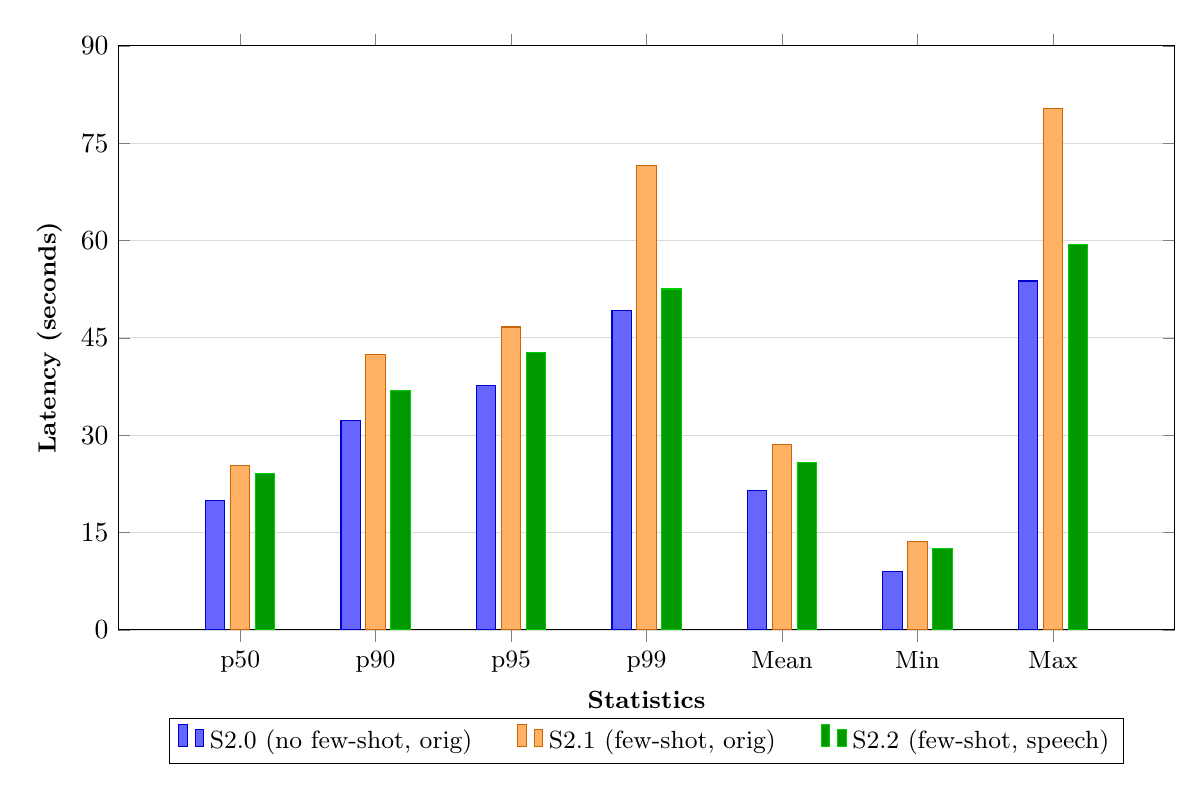
\begin{tikzpicture}
  \begin{axis}[
    width=15cm,
    height=9cm,
    ybar,
    bar width=7pt,
    ylabel={Latency (seconds)},
    ylabel style={font=\small\bfseries},
    xlabel={Statistics},
    xlabel style={font=\small\bfseries},
    symbolic x coords={p50, p90, p95, p99, Mean, Min, Max},
    xtick=data,
    xticklabel style={font=\small},
    ymin=0,
    ymax=90,
    ytick={0, 15, 30, 45, 60, 75, 90},
    ymajorgrids=true,
    grid style={line width=0.3pt, draw=gray!30},
    legend style={
      at={(0.5,-0.15)},
      anchor=north,
      legend columns=3,
      font=\small,
      /tikz/every even column/.append style={column sep=0.5cm}
    },
    enlarge x limits=0.15,
  ]
  
  % S2.0 (no few-shot, orig) - Blue
  \addplot[fill=blue!60, draw=blue!80!black] coordinates {
    (p50, 19.97)
    (p90, 32.24)
    (p95, 37.69)
    (p99, 49.26)
    (Mean, 21.48)
    (Min, 9.01)
    (Max, 53.76)
  };
  \addlegendentry{S2.0 (no few-shot, orig)}
  
  % S2.1 (few-shot, orig) - Orange
  \addplot[fill=orange!60, draw=orange!80!black] coordinates {
    (p50, 25.35)
    (p90, 42.48)
    (p95, 46.68)
    (p99, 71.52)
    (Mean, 28.58)
    (Min, 13.60)
    (Max, 80.28)
  };
  \addlegendentry{S2.1 (few-shot, orig)}
  
  % S2.2 (few-shot, speech) - Green
  \addplot[fill=green!60!black, draw=green!80!black] coordinates {
    (p50, 24.07)
    (p90, 36.93)
    (p95, 42.81)
    (p99, 52.53)
    (Mean, 25.83)
    (Min, 12.51)
    (Max, 59.36)
  };
  \addlegendentry{S2.2 (few-shot, speech)}
  
  \end{axis}
\end{tikzpicture}
\caption{Latency statistics for S2 variants (seconds).}
\label{fig:s2-latency-bar}
\end{figure}


\subsection*{Cost Analysis (S2: Single-Field Iterative)}

\textbf{Assumptions.} We extract each of the $F{=}9$ MUC-4 slots with a separate \textit{GPT-5} call. 
Per field (average): $i_f{=}1{,}500$ input tokens, $o_f{=}50$ output tokens. 
Verification with \textit{GPT-5-mini} is done \emph{once per record} (not per field) with $V_{\text{in}}{=}1{,}000$, $V_{\text{out}}{=}100$. 
If audio is used, add Whisper transcription for $D$ minutes (once per record).

\textbf{Prices.} GPT-5: input \$1.25/M, output \$10.00/M. GPT-5-mini: input \$0.25/M, output \$2.00/M. Whisper: \$0.006/min.

\textbf{Formula.}
\[
\text{Cost}_{\text{S2}} =
\underbrace{
\sum_{f=1}^{F}\!\left(\frac{i_f}{10^6}p_{\text{in}}+\frac{o_f}{10^6}p_{\text{out}}\right)
}_{\text{per-field extraction on GPT-5}}
+
\underbrace{
\frac{V_{\text{in}}}{10^6}p^{(\text{mini})}_{\text{in}}+\frac{V_{\text{out}}}{10^6}p^{(\text{mini})}_{\text{out}}
}_{\text{single verification on GPT-5-mini}}
+0.006\cdot D
\]

\textbf{Per-record (no audio).}
\[
9\times\Big(
\underbrace{\tfrac{1500}{10^6}\!\cdot\!1.25}_{\$0.001875}
+\underbrace{\tfrac{50}{10^6}\!\cdot\!10.00}_{\$0.000500}
\Big)
+\underbrace{\tfrac{1000}{10^6}\!\cdot\!0.25}_{\$0.000250}
+\underbrace{\tfrac{100}{10^6}\!\cdot\!2.00}_{\$0.000200}
=\mathbf{\$0.02183}\ (\approx 2.18\text{¢/doc})
\]

\textbf{With audio (Whisper).} Add $0.006\cdot D$. For $D{=}1$ min: $\$0.02183+0.006=\mathbf{\$0.02783}$ (\(\approx 2.78\,\text{¢}\)).

\textbf{Takeaway.} With these settings, S2 costs \(\approx 3.03\times\) S1 (\$0.02183 vs.\ \$0.00720 per doc, no audio), driven by the $F$ separate extraction calls; verification once per record keeps the verifier overhead small.



\subsection*{Insights}

\begin{itemize}
    \item \textbf{Few-shot improves accuracy and calibrates fills.} S2.1 vs.\ S2.0: OBS +0.029, SF1 +0.031; hallucinations drop substantially (HR 0.373$\rightarrow$0.301) with a small FDA gain (0.709$\rightarrow$0.718). Misses rise (MR 0.226$\rightarrow$0.267), indicating a shift toward more conservative fills.
    \item \textbf{Iterative prompting helps location.} S2.1 attains \texttt{incidentLocation} 0.597 (baseline regime), noticeably higher than S1’s single-pass numbers, consistent with field-focused instructions improving locality grounding.
    \item \textbf{Speech-style robustness with mild cost.} S2.2 maintains competitive OBS/SF1 (0.595/0.631) and similar MR to S2.1, but with lower FDA (0.700) and higher HR (0.341). RFA remains strong (0.742), suggesting good quality when both sides produce values, but overall more cautious/variable fill decisions on spoken-like inputs.
    \item \textbf{Persistent hard spot: \texttt{perpetratorIndividual}.} Scores remain low across variants due to sparse gold and ambiguous mentions; even with per-slot focus, recall lags compared to \texttt{weapon} and \texttt{perpetratorOrganization}.
    \item \textbf{Latency–quality profile.} All S2 variants are faster than the best S1 accuracy setting (S1.1). S2.0 is the speed leader (p50 $\sim$20\,s/doc) but has higher HR; S2.1 delivers the best accuracy at a moderate latency increase; S2.2 offers a middle ground for speech-like text with shorter tails than S1.1.
\end{itemize}

\section{Results – Strategy S3: Multi-LLM Consensus (Full)}
\label{sec:eval-s3}

The \textbf{S3: Multi-LLM Consensus (Full)} strategy runs multiple LLMs on the full document and aggregates with a verification/consensus step.
We evaluate three variants:
\textbf{S3.0} = no few-shot examples on the original MUC-4 dataset;
\textbf{S3.1} = with few-shot examples on the original dataset;
\textbf{S3.2} = with few-shot examples on a speech-style variant.

\subsection*{Headline Results}

% Add to your preamble:
% \usepackage{pgfplots}
% \pgfplotsset{compat=1.18}

\begin{figure}[H]
\centering
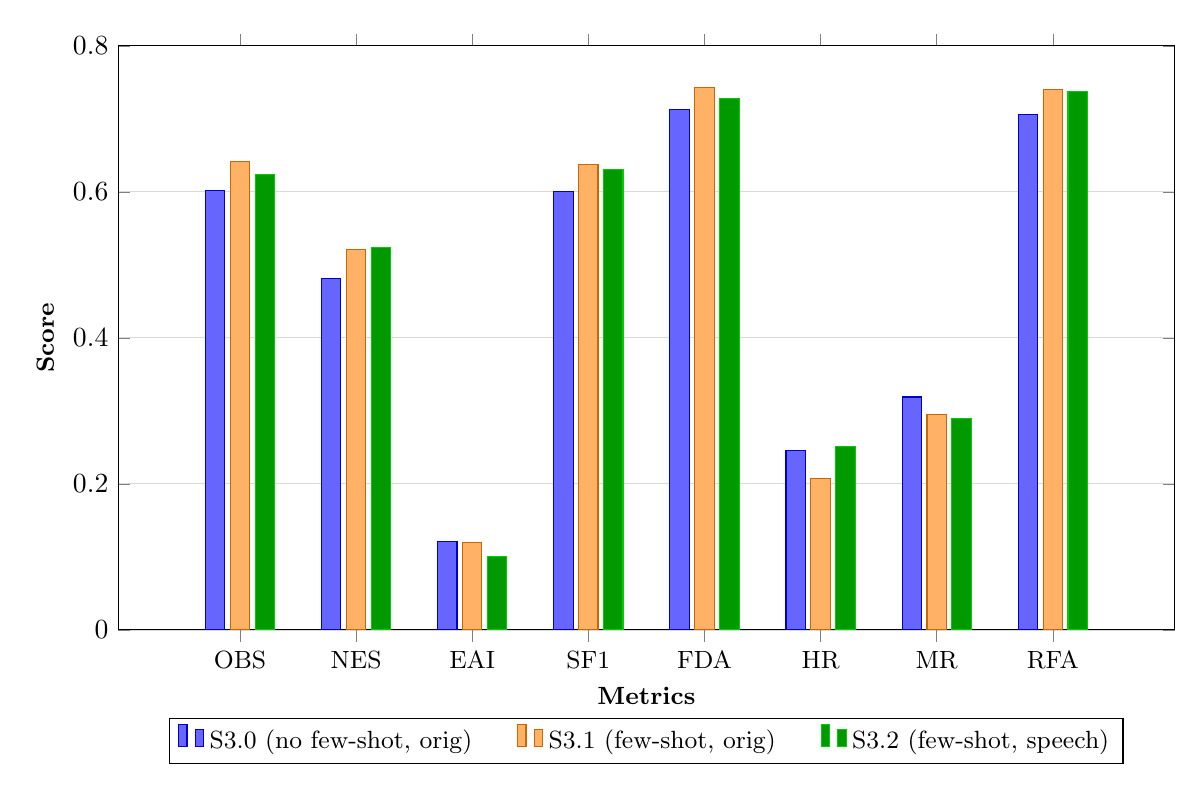
\begin{tikzpicture}
  \begin{axis}[
    width=15cm,
    height=9cm,
    ybar,
    bar width=7pt,
    ylabel={Score},
    ylabel style={font=\small\bfseries},
    xlabel={Metrics},
    xlabel style={font=\small\bfseries},
    symbolic x coords={OBS, NES, EAI, SF1, FDA, HR, MR, RFA},
    xtick=data,
    xticklabel style={font=\small},
    ymin=0,
    ymax=0.8,
    ytick={0, 0.2, 0.4, 0.6, 0.8},
    ymajorgrids=true,
    grid style={line width=0.3pt, draw=gray!30},
    legend style={
      at={(0.5,-0.15)},
      anchor=north,
      legend columns=3,
      font=\small,
      /tikz/every even column/.append style={column sep=0.5cm}
    },
    enlarge x limits=0.15,
  ]
  
  % S3.0 (no few-shot, orig) - Blue
  \addplot[fill=blue!60, draw=blue!80!black] coordinates {
    (OBS, 0.602)
    (NES, 0.481)
    (EAI, 0.121)
    (SF1, 0.601)
    (FDA, 0.713)
    (HR, 0.246)
    (MR, 0.319)
    (RFA, 0.706)
  };
  \addlegendentry{S3.0 (no few-shot, orig)}
  
  % S3.1 (few-shot, orig) - Orange
  \addplot[fill=orange!60, draw=orange!80!black] coordinates {
    (OBS, 0.641)
    (NES, 0.521)
    (EAI, 0.120)
    (SF1, 0.638)
    (FDA, 0.743)
    (HR, 0.208)
    (MR, 0.295)
    (RFA, 0.740)
  };
  \addlegendentry{S3.1 (few-shot, orig)}
  
  % S3.2 (few-shot, speech) - Green
  \addplot[fill=green!60!black, draw=green!80!black] coordinates {
    (OBS, 0.624)
    (NES, 0.524)
    (EAI, 0.100)
    (SF1, 0.630)
    (FDA, 0.728)
    (HR, 0.251)
    (MR, 0.289)
    (RFA, 0.738)
  };
  \addlegendentry{S3.2 (few-shot, speech)}
  
  \end{axis}
\end{tikzpicture}
\caption{Headline metrics for S3 variants on MUC-4 ($N{=}100$).}
\label{fig:s3-variants-bar}
\end{figure}


\paragraph{Per-field (reference for S3.1).}
Consensus is strong for \texttt{perpetratorOrganization} and \texttt{weapon}; \texttt{perpetratorIndividual} remains hardest; \texttt{incidentLocation} improves vs.\ single-pass.

\begin{table}[H]
    \centering
    \caption{Per-field average scores for S3.1 ($N{=}100$).}
    \label{tab:s3-perfield}
    \begin{tabular}{lcc}
        \toprule
        Field & Avg.\ Score & \#Docs \\
        \midrule
        incidentType & 0.510 & 100 \\
        incidentDate & 0.730 & 100 \\
        incidentLocation & 0.554 & 100 \\
        incidentStage & 0.730 & 100 \\
        perpetratorIndividual & 0.561 & 100 \\
        perpetratorOrganization & 0.756 & 100 \\
        target & 0.570 & 100 \\
        victim & 0.567 & 100 \\
        weapon & 0.793 & 100 \\
        \midrule
        \textbf{Overall (OBS)} & \textbf{0.641} & \textbf{900 comps} \\
        \bottomrule
    \end{tabular}
\end{table}

\subsection*{Latency}

\begin{figure}[H]
\centering
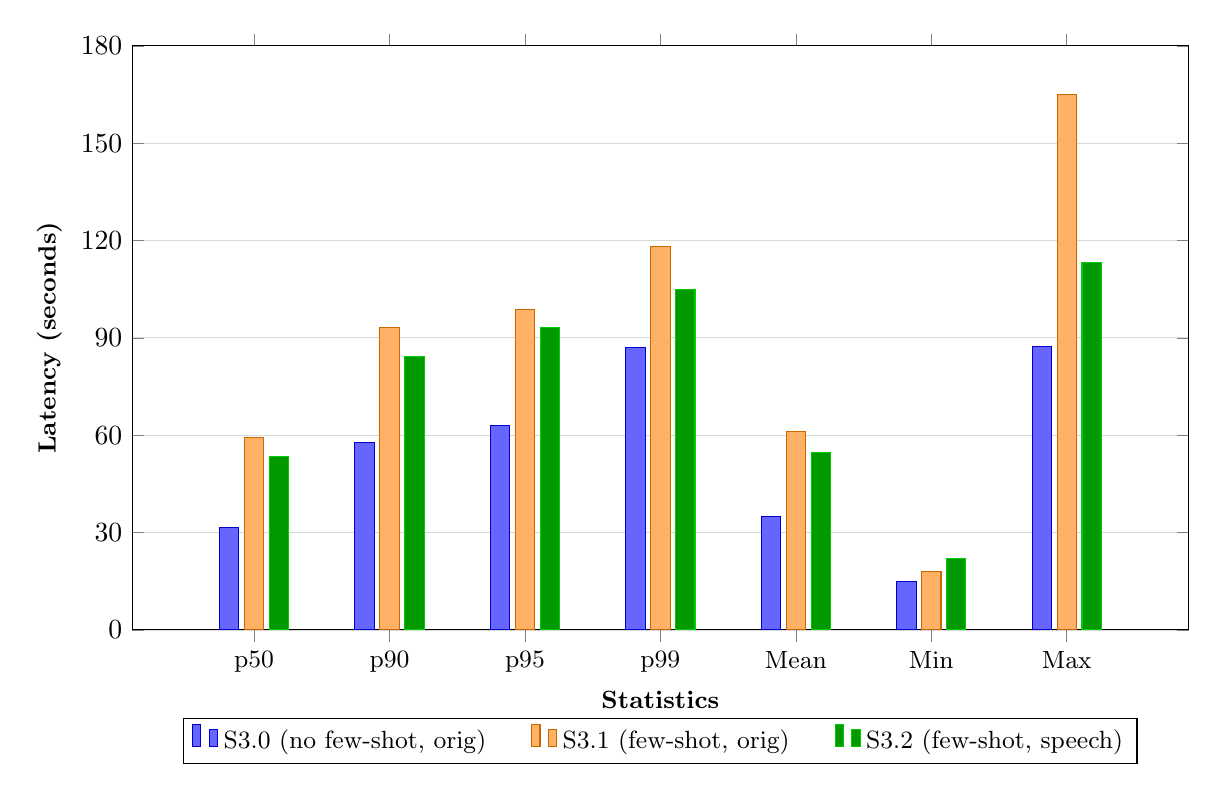
\begin{tikzpicture}
  \begin{axis}[
    width=15cm,
    height=9cm,
    ybar,
    bar width=7pt,
    ylabel={Latency (seconds)},
    ylabel style={font=\small\bfseries},
    xlabel={Statistics},
    xlabel style={font=\small\bfseries},
    symbolic x coords={p50, p90, p95, p99, Mean, Min, Max},
    xtick=data,
    xticklabel style={font=\small},
    ymin=0,
    ymax=180,
    ytick={0, 30, 60, 90, 120, 150, 180},
    ymajorgrids=true,
    grid style={line width=0.3pt, draw=gray!30},
    legend style={
      at={(0.5,-0.15)},
      anchor=north,
      legend columns=3,
      font=\small,
      /tikz/every even column/.append style={column sep=0.5cm}
    },
    enlarge x limits=0.15,
  ]
  
  % S3.0 (no few-shot, orig) - Blue
  \addplot[fill=blue!60, draw=blue!80!black] coordinates {
    (p50, 31.47)
    (p90, 57.79)
    (p95, 63.02)
    (p99, 87.16)
    (Mean, 34.83)
    (Min, 14.85)
    (Max, 87.24)
  };
  \addlegendentry{S3.0 (no few-shot, orig)}
  
  % S3.1 (few-shot, orig) - Orange
  \addplot[fill=orange!60, draw=orange!80!black] coordinates {
    (p50, 59.39)
    (p90, 93.15)
    (p95, 98.77)
    (p99, 118.28)
    (Mean, 61.09)
    (Min, 18.13)
    (Max, 164.96)
  };
  \addlegendentry{S3.1 (few-shot, orig)}
  
  % S3.2 (few-shot, speech) - Green
  \addplot[fill=green!60!black, draw=green!80!black] coordinates {
    (p50, 53.45)
    (p90, 84.15)
    (p95, 93.31)
    (p99, 104.99)
    (Mean, 54.55)
    (Min, 22.01)
    (Max, 113.26)
  };
  \addlegendentry{S3.2 (few-shot, speech)}
  
  \end{axis}
\end{tikzpicture}
\caption{Latency statistics for S3 variants (seconds).}
\label{fig:s3-latency-bar}
\end{figure}

\subsection*{Insights}

\begin{itemize}
    \item \textbf{Consensus cuts hallucinations and improves calibration.} Relative to iterative S2.1, S3.1 lowers HR (0.301$\rightarrow$0.208) and raises FDA (0.718$\rightarrow$0.743), with higher OBS (+0.022) at a modest MR increase (0.267$\rightarrow$0.295). This reflects better confidence alignment from cross-model agreement.
    \item \textbf{Competitive with the best single-pass accuracy.} Against S1.1, S3.1 is close on OBS (0.641 vs.\ 0.644) but improves NES (0.521 vs.\ 0.504), suggesting stronger content quality on gold-nonempty fields; MR also improves (0.295 vs.\ 0.313), while HR is slightly higher than S1.1’s very conservative rate (0.208 vs.\ 0.180).
    \item \textbf{Speech-style robustness holds.} S3.2 maintains NES leadership among S3 variants (0.524) and strong RFA (0.738), with MR the lowest (0.289). Compared to S1.2, S3.2 trades a small OBS deficit (0.624 vs.\ 0.626) for better NES (+0.016) and similar FDA (0.728 vs.\ 0.727).
    \item \textbf{Field patterns persist.} \texttt{perpetratorOrganization}/\texttt{weapon} remain easiest; \texttt{perpetratorIndividual} continues to lag due to sparse, ambiguous references; \texttt{incidentLocation} benefits from full-context cross-checking (S3.1: 0.554 baseline) vs.\ S1’s single pass.
    \item \textbf{Latency cost is real but tails are reasonable.} S3.1 has higher median and mean than S1.1, yet a shorter extreme tail than S1.1 (p99 118.3\,s vs.\ 134.9\,s). S3.0 offers a faster consensus baseline when few-shot is unavailable.
\end{itemize}

\section{Results – Strategy S4: Multi-LLM Per-Field}
\label{sec:eval-s4}

The \textbf{S4: Multi-LLM Per-Field} strategy applies consensus at the slot level: each field is extracted by multiple models and consolidated via a field-aware verifier. We evaluate:
\textbf{S4.0} = no few-shot on the original MUC-4 dataset;
\textbf{S4.1} = few-shot on the original dataset;
\textbf{S4.2} = few-shot on a speech-style variant.

\subsection*{Headline Results}

\begin{table}[h]
    \centering
    \caption{Headline metrics for S4 variants on MUC-4 ($N{=}100$).}
    \label{tab:s4-variants-headline}
    \begin{tabular}{lcccccccc}
        \toprule
        Variant & OBS & NES & EAI & SF1 & FDA & HR & MR & RFA \\
        \midrule
        S4.0 (no few-shot, orig) & 0.549 & \textbf{0.628} & \textbf{-0.080} & 0.589 & 0.693 & \textbf{0.551} & \textbf{0.112} & 0.708 \\
        S4.1 (few-shot, orig)    & \textbf{0.579} & 0.624 & -0.044 & \textbf{0.613} & \textbf{0.709} & 0.476 & 0.144 & \textbf{0.728} \\
        S4.2 (few-shot, speech)  & 0.572 & 0.612 & -0.040 & 0.592 & 0.704 & 0.479 & 0.150 & 0.719 \\
        \bottomrule
    \end{tabular}
\end{table}

\paragraph{Per-field (reference for S4.1).}
Per-field consensus boosts \texttt{incidentLocation}; \texttt{perpetratorIndividual} remains hardest; \texttt{weapon} is lower than S1/S3.

\begin{table}[H]
    \centering
    \caption{Per-field average scores for S4.1 ($N{=}100$).}
    \label{tab:s4-perfield}
    \begin{tabular}{lcc}
        \toprule
        Field & Avg.\ Score & \#Docs \\
        \midrule
        incidentType & 0.440 & 100 \\
        incidentDate & 0.370 & 100 \\
        incidentLocation & 0.641 & 100 \\
        incidentStage & 0.720 & 100 \\
        perpetratorIndividual & 0.585 & 100 \\
        perpetratorOrganization & 0.644 & 100 \\
        target & 0.550 & 100 \\
        victim & 0.572 & 100 \\
        weapon & 0.692 & 100 \\
        \midrule
        \textbf{Overall (OBS)} & \textbf{0.579} & \textbf{900 comps} \\
        \bottomrule
    \end{tabular}
\end{table}

\subsection*{Latency}

\begin{table}[H]
    \centering
    \caption{Latency statistics for S4 variants (seconds).}
    \label{tab:s4-latency-all}
    \begin{tabular}{lccccccc}
        \toprule
        Variant & p50 & p90 & p95 & p99 & Mean & Min & Max \\
        \midrule
        S4.0 (no few-shot, orig) & 125.14 & 157.96 & 166.02 & 177.27 & 128.64 & 97.08 & 179.00 \\
        S4.1 (few-shot, orig)    & 121.81 & 143.39 & 155.16 & 164.08 & 124.98 & 98.10 & 168.81 \\
        S4.2 (few-shot, speech)  & \textbf{127.23} & \textbf{159.02} & \textbf{175.50} & \textbf{192.16} & \textbf{131.15} & \textbf{84.42} & \textbf{218.22} \\
        \bottomrule
    \end{tabular}
\end{table}

\subsection*{Insights}

\begin{itemize}
    \item \textbf{Per-field consensus is aggressive: high NES, negative EAI.} All S4 variants show NES $\geq$ 0.612 with \emph{negative} EAI (e.g., S4.1: $-0.044$), meaning they excel when gold is nonempty but overfill when gold is empty. This matches the high HR (0.476–0.551) coupled with very low MR (0.112–0.150).
    \item \textbf{Few-shot moderates overfilling and lifts quality.} S4.1 vs.\ S4.0 raises OBS (+0.030) and SF1 (+0.025), reduces HR (0.551$\rightarrow$0.476), and slightly increases MR (0.112$\rightarrow$0.144) — shifting toward more calibrated fills while keeping RFA high (0.728).
    \item \textbf{Speech-style robustness is steady but cautious.} S4.2 keeps strong NES (0.612) and similar FDA (0.704) to S4.1, with a small OBS/SF1 drop and modestly higher MR (0.150). RFA remains solid (0.719), indicating good quality when both sides fill.
    \item \textbf{Field-level effects.} \texttt{incidentLocation} benefits most from per-slot consensus (S4.1: 0.641), surpassing single-pass baselines. \texttt{weapon} lags S1/S3 (0.692 in S4.1), suggesting per-field voting can over-accept marginal mentions; \texttt{perpetratorIndividual} remains the hardest across strategies.
    \item \textbf{Compared to S3 (full-document consensus).} S4.1 has much higher NES (0.624 vs.\ 0.521 for S3.1) but lower OBS (0.579 vs.\ 0.641) due to higher HR. In short: S4 is great when the slot truly exists, but its aggressiveness hurts overall scoring when gold is empty.
    \item \textbf{Latency is the trade-off frontier.} S4 is the slowest family by design (p50 $\approx$ 122–127\,s/doc; tails reaching 160–190\,s). If throughput matters, S3.1 offers a better accuracy–latency balance; if maximizing filled content on nonempty fields is key, S4.1 is attractive with careful post-filters.
\end{itemize}

\section{Comparative Analysis of Strategies}
\label{sec:eval-comparative}

We compare four \textit{Invox} strategies—S1 (single-pass), S2 (iterative per-field), S3 (full-document consensus), and S4 (per-field consensus)—along \textbf{semantic accuracy} (R2), \textbf{latency} (R6), and \textbf{modularity} (R5). 
All numbers below use the few-shot, original MUC-4 setting for each strategy.

\subsection*{Quantitative Comparison}

% Add to your preamble:
% \usepackage{pgfplots}
% \pgfplotsset{compat=1.18}

\begin{figure}[h]
\centering
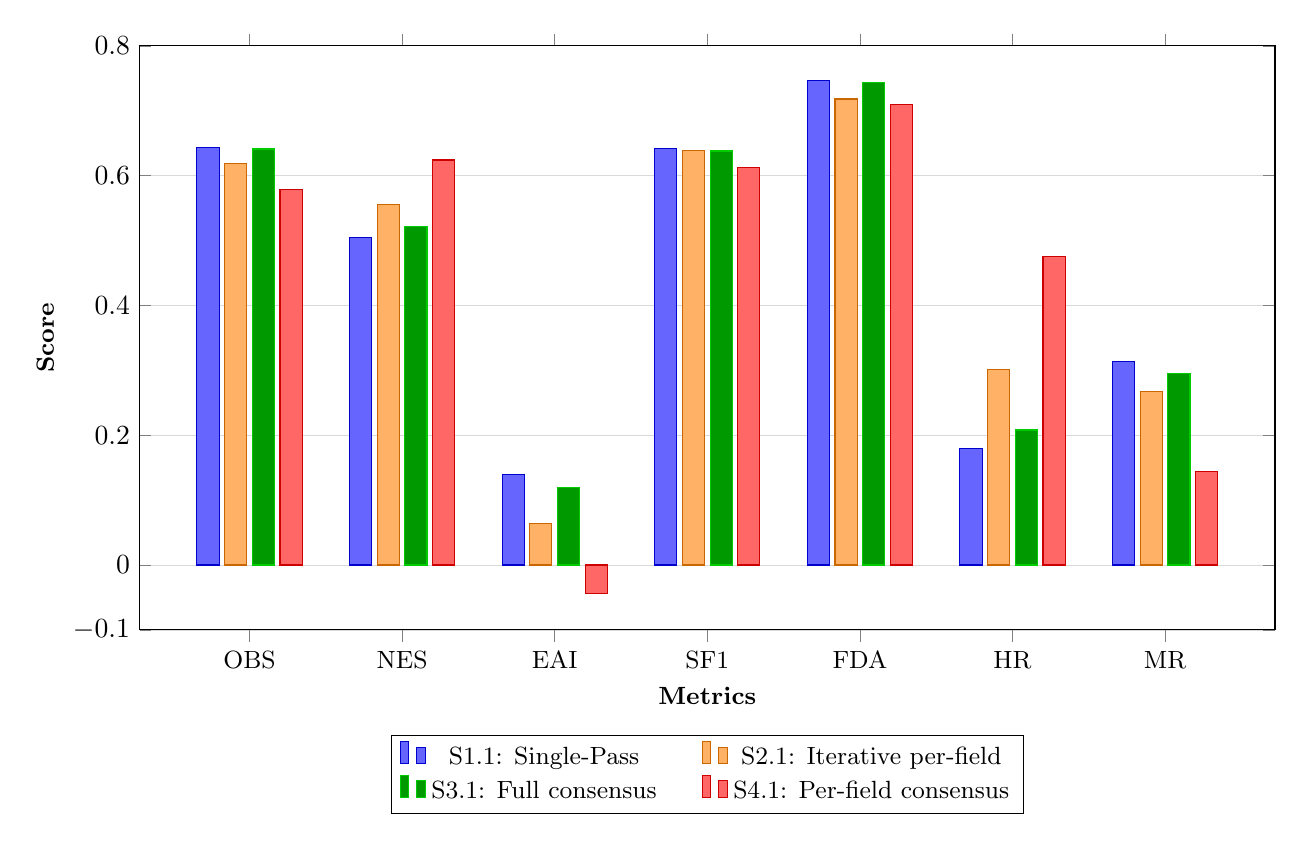
\begin{tikzpicture}
  \begin{axis}[
    width=16cm,
    height=9cm,
    ybar,
    bar width=8pt,
    ylabel={Score},
    ylabel style={font=\small\bfseries},
    xlabel={Metrics},
    xlabel style={font=\small\bfseries},
    symbolic x coords={OBS, NES, EAI, SF1, FDA, HR, MR},
    xtick=data,
    xticklabel style={font=\small},
    ymin=-0.1,
    ymax=0.8,
    ytick={-0.1, 0, 0.2, 0.4, 0.6, 0.8},
    ymajorgrids=true,
    grid style={line width=0.3pt, draw=gray!30},
    legend style={
      at={(0.5,-0.18)},
      anchor=north,
      legend columns=2,
      font=\small,
      /tikz/every even column/.append style={column sep=0.5cm}
    },
    enlarge x limits=0.12,
  ]
  
  % S1.1: Single-Pass - Blue
  \addplot[fill=blue!60, draw=blue!80!black] coordinates {
    (OBS, 0.644)
    (NES, 0.504)
    (EAI, 0.140)
    (SF1, 0.642)
    (FDA, 0.746)
    (HR, 0.180)
    (MR, 0.313)
  };
  \addlegendentry{S1.1: Single-Pass}
  
  % S2.1: Iterative per-field - Orange
  \addplot[fill=orange!60, draw=orange!80!black] coordinates {
    (OBS, 0.619)
    (NES, 0.555)
    (EAI, 0.064)
    (SF1, 0.639)
    (FDA, 0.718)
    (HR, 0.301)
    (MR, 0.267)
  };
  \addlegendentry{S2.1: Iterative per-field}
  
  % S3.1: Full consensus - Green
  \addplot[fill=green!60!black, draw=green!80!black] coordinates {
    (OBS, 0.641)
    (NES, 0.521)
    (EAI, 0.120)
    (SF1, 0.638)
    (FDA, 0.743)
    (HR, 0.208)
    (MR, 0.295)
  };
  \addlegendentry{S3.1: Full consensus}
  
  % S4.1: Per-field consensus - Red
  \addplot[fill=red!60, draw=red!80!black] coordinates {
    (OBS, 0.579)
    (NES, 0.624)
    (EAI, -0.044)
    (SF1, 0.613)
    (FDA, 0.709)
    (HR, 0.476)
    (MR, 0.144)
  };
  \addlegendentry{S4.1: Per-field consensus}
  
  \end{axis}
\end{tikzpicture}
\caption{Macro comparison (clean text; few-shot original).}
\label{fig:strategy-comparison-bar}
\end{figure}

\noindent\textit{Embedding alignment (baseline regime):} Chamfer (sym.) — S1.1: 0.642; S2.1: 0.639; S3.1: 0.638; S4.1: 0.613.

\subsection*{Latency Comparison (R6)}
\begin{figure}[h]
\centering
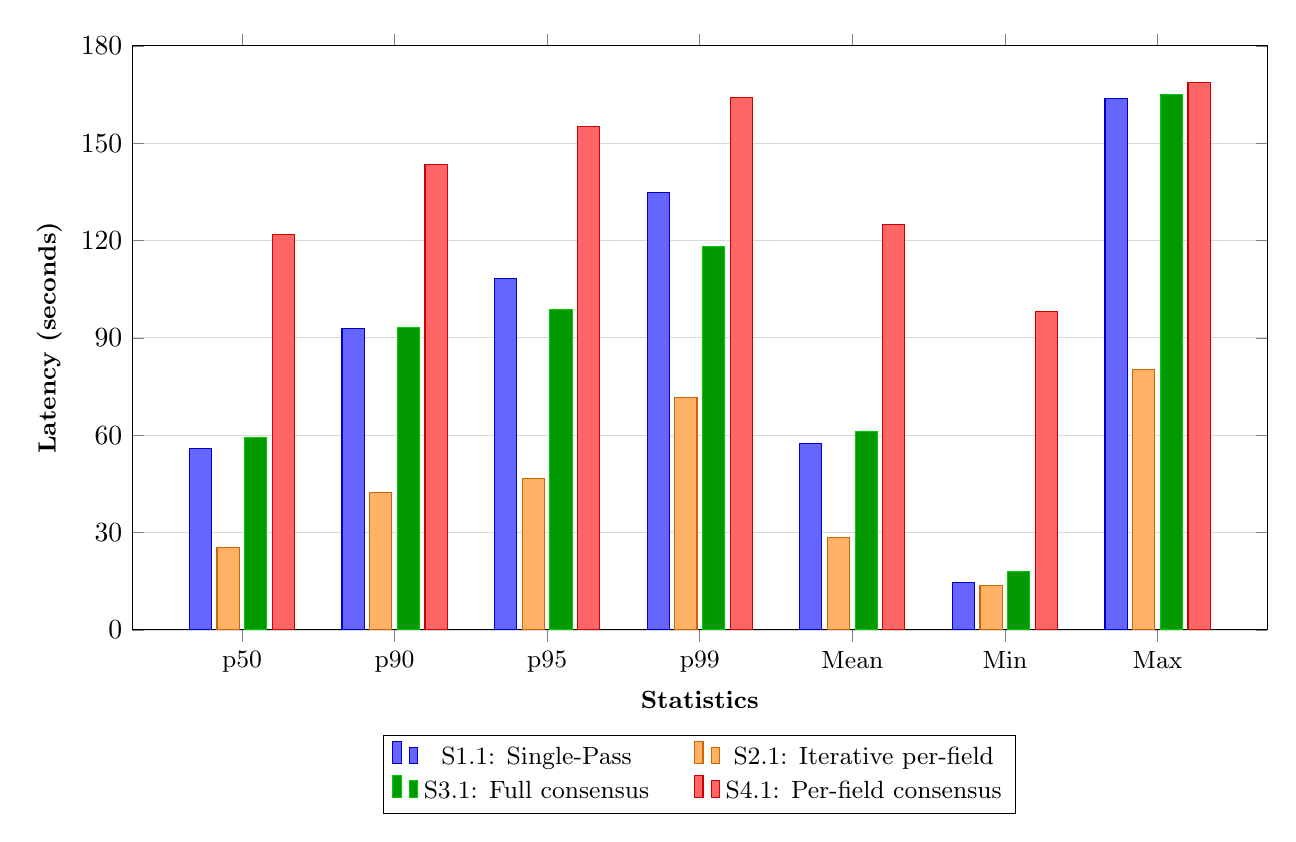
\begin{tikzpicture}
  \begin{axis}[
    width=16cm,
    height=9cm,
    ybar,
    bar width=8pt,
    ylabel={Latency (seconds)},
    ylabel style={font=\small\bfseries},
    xlabel={Statistics},
    xlabel style={font=\small\bfseries},
    symbolic x coords={p50, p90, p95, p99, Mean, Min, Max},
    xtick=data,
    xticklabel style={font=\small},
    ymin=0,
    ymax=180,
    ytick={0, 30, 60, 90, 120, 150, 180},
    ymajorgrids=true,
    grid style={line width=0.3pt, draw=gray!30},
    legend style={
      at={(0.5,-0.18)},
      anchor=north,
      legend columns=2,
      font=\small,
      /tikz/every even column/.append style={column sep=0.5cm}
    },
    enlarge x limits=0.12,
  ]
  
  % S1.1: Single-Pass - Blue
  \addplot[fill=blue!60, draw=blue!80!black] coordinates {
    (p50, 55.91)
    (p90, 93.01)
    (p95, 108.40)
    (p99, 134.93)
    (Mean, 57.34)
    (Min, 14.54)
    (Max, 163.79)
  };
  \addlegendentry{S1.1: Single-Pass}
  
  % S2.1: Iterative per-field - Orange
  \addplot[fill=orange!60, draw=orange!80!black] coordinates {
    (p50, 25.35)
    (p90, 42.48)
    (p95, 46.68)
    (p99, 71.52)
    (Mean, 28.58)
    (Min, 13.60)
    (Max, 80.28)
  };
  \addlegendentry{S2.1: Iterative per-field}
  
  % S3.1: Full consensus - Green
  \addplot[fill=green!60!black, draw=green!80!black] coordinates {
    (p50, 59.39)
    (p90, 93.15)
    (p95, 98.77)
    (p99, 118.28)
    (Mean, 61.09)
    (Min, 18.13)
    (Max, 164.96)
  };
  \addlegendentry{S3.1: Full consensus}
  
  % S4.1: Per-field consensus - Red
  \addplot[fill=red!60, draw=red!80!black] coordinates {
    (p50, 121.81)
    (p90, 143.39)
    (p95, 155.16)
    (p99, 164.08)
    (Mean, 124.98)
    (Min, 98.10)
    (Max, 168.81)
  };
  \addlegendentry{S4.1: Per-field consensus}
  
  \end{axis}
\end{tikzpicture}
\caption{Latency profile (seconds; clean text).}
\label{fig:latency-comparison-bar}
\end{figure}


\subsection*{Insights}

\begin{itemize}
    \item \textbf{Best overall accuracy on clean text:} \underline{S1.1} leads OBS (0.644) and SF1 (0.642), with the lowest HR (0.180) and the highest FDA (0.746). Strong default when you want accuracy with minimal orchestration.
    \item \textbf{Quality when gold is nonempty:} \underline{S4.1} tops NES (0.624) and has the lowest MR (0.144), but does so via aggressive filling (HR 0.476), lowering its OBS.
    \item \textbf{Calibration via consensus:} \underline{S3.1} is near S1.1 on OBS (0.641 vs.\ 0.644) while improving NES (0.521 vs.\ 0.504) and FDA (0.743), and cutting HR vs.\ S2.1 (0.208 vs.\ 0.301). A strong choice when you want additional stability without a huge latency jump over S1.
    \item \textbf{Throughput leader with solid accuracy:} \underline{S2.1} is the fastest (p50 25.35s) and improves field grounding (e.g., location), trading a modest OBS drop and higher HR for speed and interpretability.
    \item \textbf{Latency hierarchy:} S2.1 \(\rightarrow\) S1.1 \(\approx\) S3.1 \(\rightarrow\) S4.1. Use S4.1 only when maximizing fills on known-present slots is key and you can post-filter to curb overfilling.
\end{itemize}


\subsection*{Summary}

\begin{itemize}
    \item \textbf{S1.1} = best single-model accuracy and calibration on clean text.
    \item \textbf{S3.1} = consensus-calibrated stability with near-S1 accuracy.
    \item \textbf{S2.1} = best latency with competitive accuracy and clearer per-field control.
    \item \textbf{S4.1} = highest NES/lowest MR but overfills; apply verification/post-filters.
\end{itemize}


